The measurement results of the processed devices obtained using the THz-TDS setup are presented below. Since some of the processed antennas share identical geometries, only the most notable antennas are discussed here. A complete set of measurements is provided in the appendix. The processed H-dipole antennas are DC-characterized. This provides insight into the overall quality of the fabricated devices and verifies whether the assumptions made in the simulations for NiCr-modified antennas hold true. The effect of adding NiCr to the devices on the time-domain measurements is briefly investigated. A comparative study of the received time-domain THz signal as well as the power spectrum based on antenna geometry is presented for H-Dipole and I-shaped Dipole antennas. H-Dipoles and I-shaped Dipoles are also evaluated in terms of received THz signal and power spectrum based on their overall topology. 

\subsection{DC Characterization}

% \begin{itemize}
%     \item talk about short circuit plots --> resistance higher than expected; calculate sheet resistance from measurements to apply to I-shaped Dipoles 
%     \item also include IV-char. of H-Dipoles and Dipoles (could be too many plots though, maybe just put in appendix)
% \end{itemize}

The fabricated antennas are DC characterized by taking their dark IV characteristics. The behavior of the dark current over a DC supply voltage gives insight on the general quality of the devices. Features we look for are: 
\begin{enumerate}
    \item dark IV curves that are mostly linear in a given biasing range, ensuring an ohmic contact, 
    \item a low dark current, reducing the overall noise of the devices. 
\end{enumerate}

We also aim to calculate the actual resistance and sheet resistance of NiCr in the fabricated devices. The resistance of NiCr is determined by measuring the short circuit current of the processed H-Dipole antennas which feature NiCr segments of different length. 

\subsubsection{Dark IV-Characterization}

The IV-characteristics of the processed H-Dipole and I-shaped Dipole antennas are taken by applying a DC bias to the devices pads. The biasing voltage ranges from \num{-1000}\,\si{\milli \volt} to \num{1000}\,\si{\milli \volt}. This biasing range is sufficient to evaluate the quality of the contact between the metal and the semiconducting substrate. The antennas are used exclusively as receivers in the measurements, with the bias provided by the incident THz field. Dark current measurements are taken in \num{50}\,\si{\milli \volt} steps. Figure \ref{iv} shows the dark IV curves for H-Dipoles (see Figure \ref{iv_HD}) and I-shaped Dipoles (see Figure \ref{iv_D}). For both antennas, linear curves are observed, indicating an ohmic contact. InGaAs substrates typically exhibit a dark resistance in the \num{1}\,\si{\mega \ohm} range \cite{seddonContinuousWaveTerahertz2024}. The mean dark resistance for the H-Dipoles is \num{612.899}\,\si{\kilo \ohm}. For the I-shaped Dipoles, the mean dark resistances is \num{3689.520}\,\si{\kilo \ohm}. Differences in dark resistance may arise from substrate inhomogeneities, material imperfections, variations in the fabrication process, or even differences in antenna geometry. The different dark resistances are expected to influence THz measurements. A larger dark resistance is generally associated with less noise. A vital noise source is thermal noise, where the effective noise current is 
\begin{equation}
    I_{n, eff} = \sqrt{\frac{4k_B T \Delta \nu}{R}} \sim \sqrt{\frac{1}{R}}.
\end{equation}

Here, $k_b$ is the Boltzmann constant, $T$ is the temperature, and $\Delta \nu$ is the frequency range. The effective noise current due to thermal noise decreases with increasing dark resistance. Other noise sources include laser intensity fluctuations, timing jitter between laser pulses, seismic vibrations, and electronic noise from the amplifier \cite{dongNoiseCharacteristicsTerahertz2015,vanexterCharacterizationOptoelectronicTerahertz1990}. Except for thermal noise, all other noise contributions are expected to be similar across measurements. Therefore, the I-shaped Dipoles are expected to exhibit lower overall noise, resulting in a higher DNR.

\begin{figure}[!]
    \centering
    \begin{subfigure}[b]{0.49\textwidth}
        \centering
        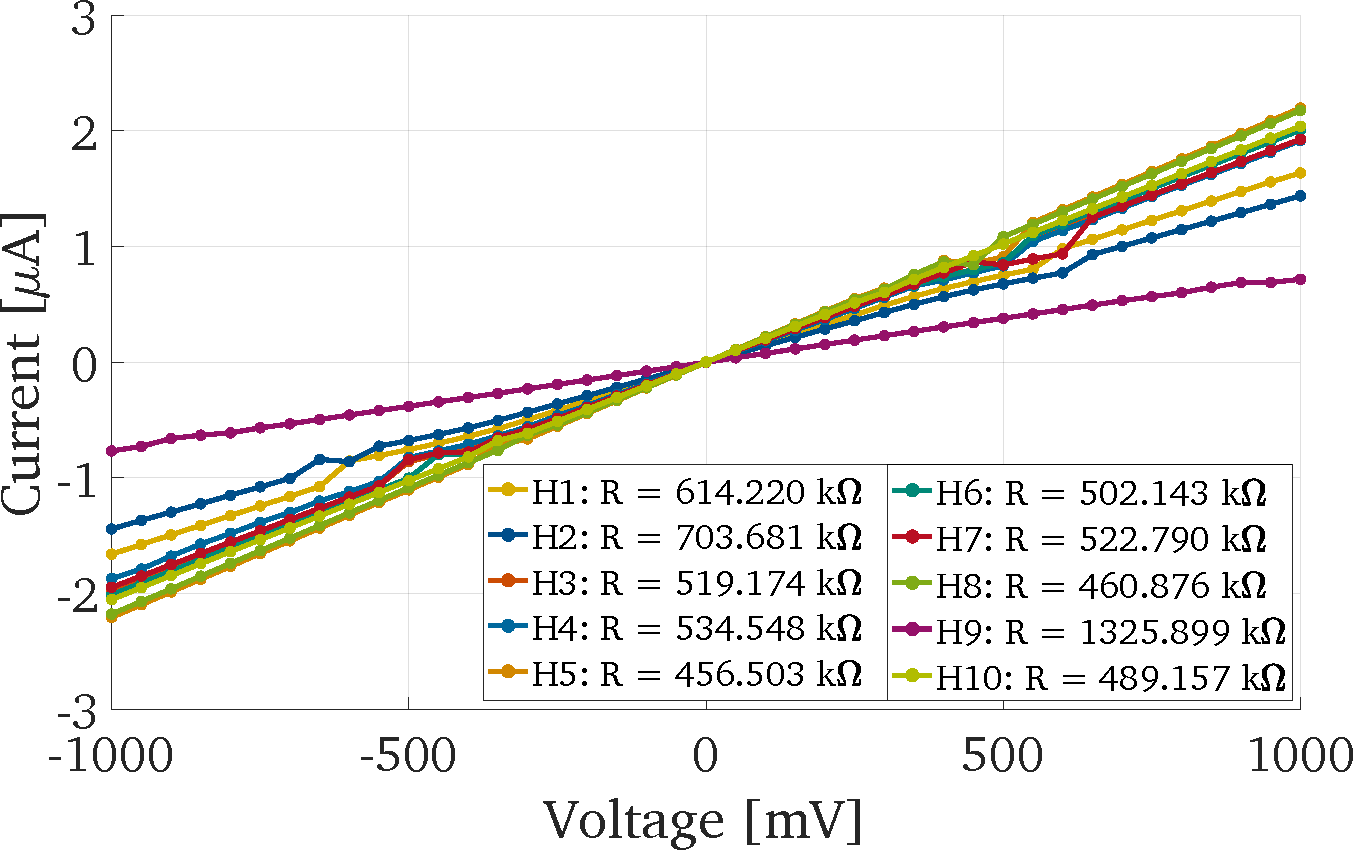
\includegraphics[height=0.6\textwidth]{figures/IV_v3/IV_H_Dipoles.pdf}
        \caption{\centering
        H-Dipole antennas}
        \label{iv_HD}
    \end{subfigure}
    \hfill
    \begin{subfigure}[b]{0.49\textwidth}
        \centering
        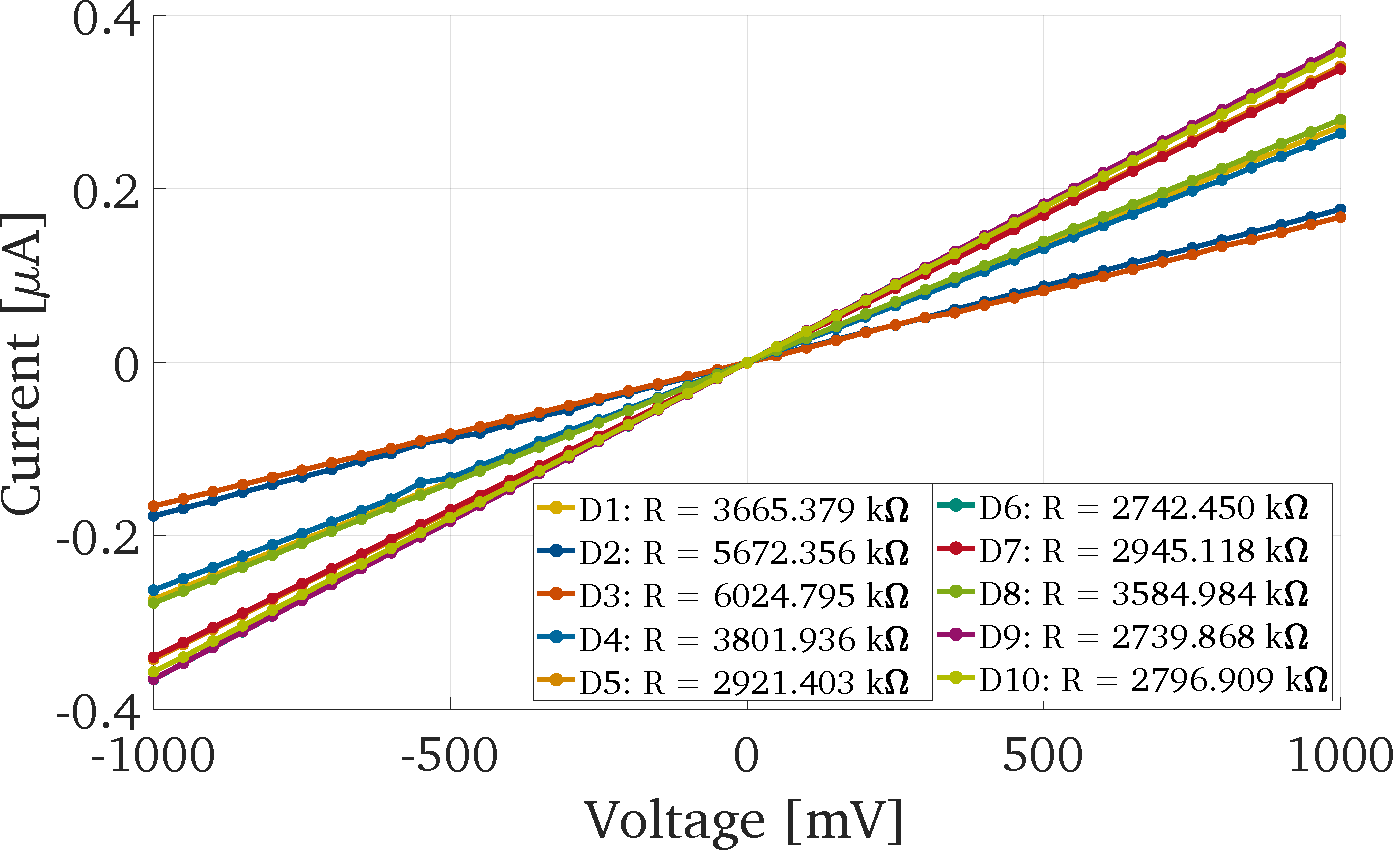
\includegraphics[height=0.6\textwidth]{figures/IV_v3/IV_I_Dipoles.pdf}
        \caption{\centering
        I-shaped Dipole antennas}
        \label{iv_D}
    \end{subfigure}
    \caption{The dark IV curves for the processed antennas are displayed. (a) Dark IV curves of H-Dipole antennas. (b) Dark IV curves of I-shaped Dipole antennas.}
    \label{iv}
\end{figure}

\subsubsection{Determination of NiCR Sheet Resistance}

% \begin{wrapfigure}{r}{0.5\textwidth} 
%     \centering
%     \captionsetup{width=0.45\textwidth}
%     \begin{tabular}{|c|c|c|c|c|}
%         \hline
%         Sample & R\textsubscript{meas} [\si{\ohm}] & W/L & R\textsubscript{sh} [\si{\ohm}/sq]\\
%         \hline
%         H4 & 5439 & 1/2 & 2719.5 \\
%         H2 & 14402 & 1/4 & 3600.5 \\
%         H6 & 15300 & 1/6 & 2550.0 \\
%         H3 & 30625 & 1/28 & 1094.7 \\
%         H8 & 15369 & 1/28 & 548.9 \\
%         H7 & 44615 & 1/96 & 464.6 \\
%         \hline
%     \end{tabular}
%     \caption{Calculations of sheet resistances for NiCr segments from measured short-circuit currents.}
%     \label{tab:sheetres}
% \end{wrapfigure}

\begin{wrapfigure}{r}{0.5\textwidth} % r = right side, 50% of text width
    \centering
    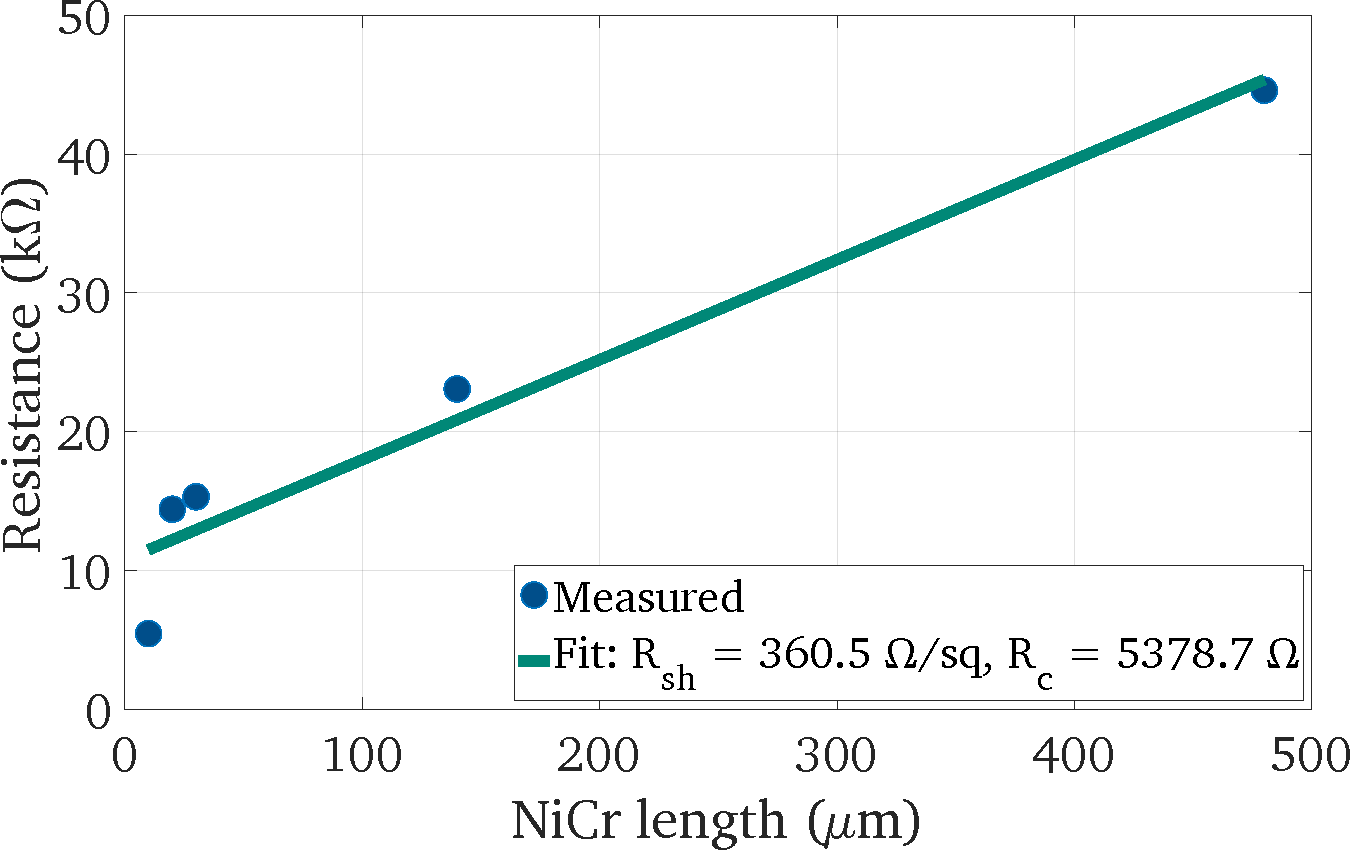
\includegraphics[width=0.49\textwidth]{figures/R_sheet_regression.pdf}
    \captionsetup{width=0.475\textwidth} % caption matches image width
    \caption{Linear fit of the measured resistances of NiCr segments introduced to an H-Dipole's feeding strip.}
    \label{fig:Rsheet:reg}
\end{wrapfigure}

By shorting one of the H-Dipoles feeding strips connected to two read-out pads, we can determine the resistance of the NiCr segments. Figure \ref{iv_sc} shows the measured short-circuit dark currents $I_{DC}$ over the applied bias voltage. The H-Dipoles with added NiCr segments are biased from \num{-20}\,\si{\milli \volt} to \num{20}\,\si{\milli \volt}. The H-Dipoles without added NiCr (see \ref{sc_wo_Nicr}) segments are biased from \num{-8}\,\si{\milli \volt} to \num{8}\,\si{\milli \volt} to avoid heating and potential damage. From Figure \ref{sc_wo_Nicr} it can be seen that the influence of the CrAu strip on NiCr resistance calculations is negligible. The resistance of the strip made solely from CrAu measures approx. \num{80}\,\si{\ohm}. The resistances of the NiCr-modified antennas lie in the \num{10}\,\si{\kilo \ohm} range. Using these measurements lets us determine the actual sheet resistance of the \num{80}/\num{20} NiCr alloy that was used in the fabrication process. The measured resistance $R_{meas}$ and sheet resistance $R_{sh}$ of NiCr relate as following: 
\begin{equation}
    R_{meas} = R_{sh}\frac{L}{W}
\end{equation}


where $W$ and $L$  are the width and the length of the NiCr segment respectively. Note that $L$ is defined as $L = 2l_{NiCr}$, as one antenna feeding strip contains two NiCr sections. The sheet resistances for each antenna containing NiCr segments are 
are calculated by linearly fitting the measured data (see Figure \ref{fig:Rsheet:reg}). Note that as two antennas with NiCr segments of length \num{70}\,\si{\micro \meter} were measured, the mean of the two measurements is used for further calculations. The linear fit returns the slope of the Resistance over NiCr length, corresponding to the sheet resistance of the NiCr alloy. We get a value of $R_{sh} = 360.5$\,\si{\ohm}/sq, as well as a factor $R_c = 5378.7$\,\si{\ohm}. The goodness of the fit is $R^2 = 0.9402$. The calculated sheet resistance lets us approximate the resistance of the NiCr segments in the I-shaped Dipole antennas using $R_{NiCr} = R_{sh}\frac{L}{W}$. As the I-shaped Dipoles cannot be shorted we cannot determine the resistance of the NiCr segments directly. Approximating the resistance in the I-shaped Dipoles using the calculated sheet resistance gives us insight into the influence of the resistance on THz measurements.

The measured value differs from the value used in simulations by a factor of \num{16}. The antennas were initially designed assuming a sheet resistance of \num{22}\,\si{\ohm}/sq. The high resistances incorporated into the antennas influence the time-domain measurements as they introduce highly dissipative elements. The exact reasons for the discrepancy between expected and actual sheet resistance require further investigation. One contributing factor is the dependence of NiCr sheet resistance on film thickness. The NiCr segments were deposited with a thickness of approx. \num{35}\,\si{\nano \meter}. The sheet resistance of thin films increases exponentially with decreasing film thickness \cite{wittElectromechanicalPropertiesThin1974}. One study of \num{80}/\num{20} NiCr alloys found the sheet resistance at \num{35}\,\si{\nano \meter} to be approx. \num{130}\,\si{\ohm}/sq. Another study reported values of up to \num{175}\,\si{\ohm}/sq. Additional sources of deviation include the evaporation rate and actual NiCR composition \cite{rolkeNichromeThinFilm1981}, as well as the contact resistance between the NiCr and CrAu segments \cite{zhangAnalysisCurrentCrowding2015} The contact resistance was partly accounted for in calculation of the sheet resistance as the correction factor $R_c$. 

\begin{figure}[!]
    \centering
    \begin{subfigure}[b]{0.49\textwidth}
        \centering
        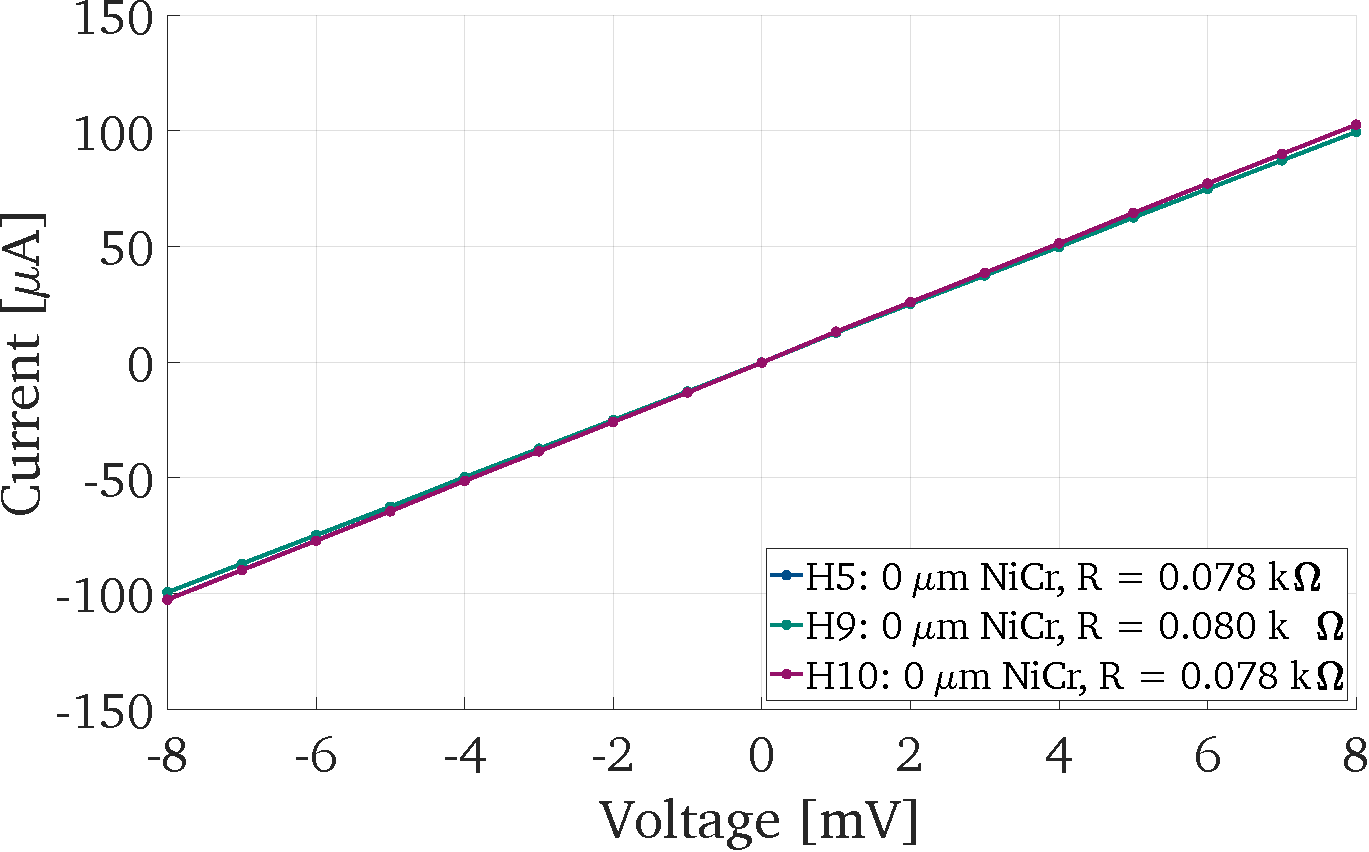
\includegraphics[height=0.6\textwidth]{figures/IV_v3/sc_h5_h9_h10.pdf}
        \caption{\centering
        H-Dipoles without added NiCr}
        \label{sc_wo_Nicr}
    \end{subfigure}
    \hfill
    \begin{subfigure}[b]{0.49\textwidth}
        \centering
        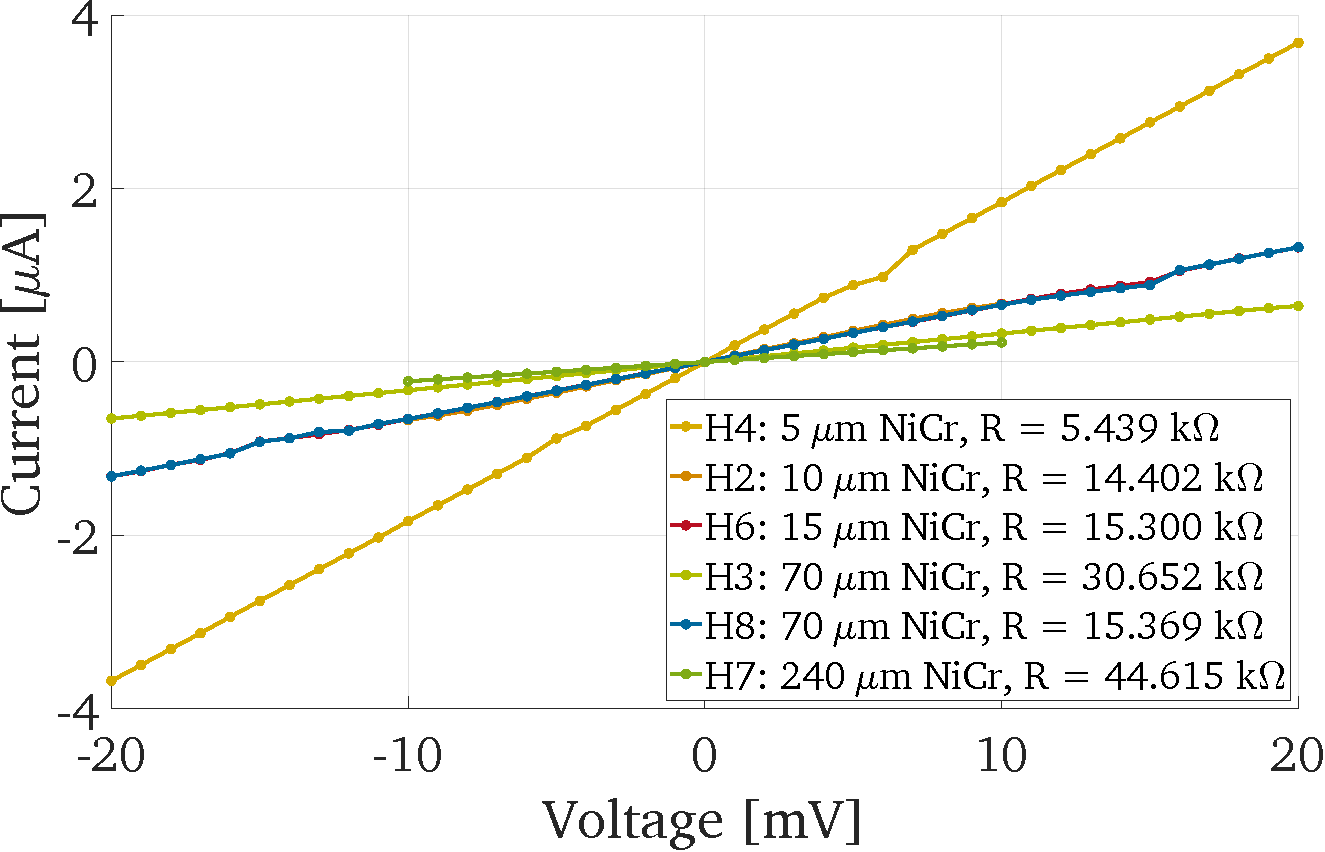
\includegraphics[height=0.6\textwidth]{figures/IV_v3/sc_h_dipoles_nicr.pdf}
        \caption{\centering
        H-Dipoles with added NiCr}
        \label{sc_w_NiCr}
    \end{subfigure}
    \caption{The short circuit current in H-Dipole antennas is displayed. (a) Short circuit resistance for H-Dipoles without NiCr segments. (b) Short circuit resistance for H-Dipoles with added NiCr segments.}
    \label{iv_sc}
\end{figure}

\subsection{Effect of NiCr on Time-Domain THz Measurements}

\begin{figure}[!]
    \centering
    \begin{subfigure}[b]{0.49\textwidth}
        \centering
        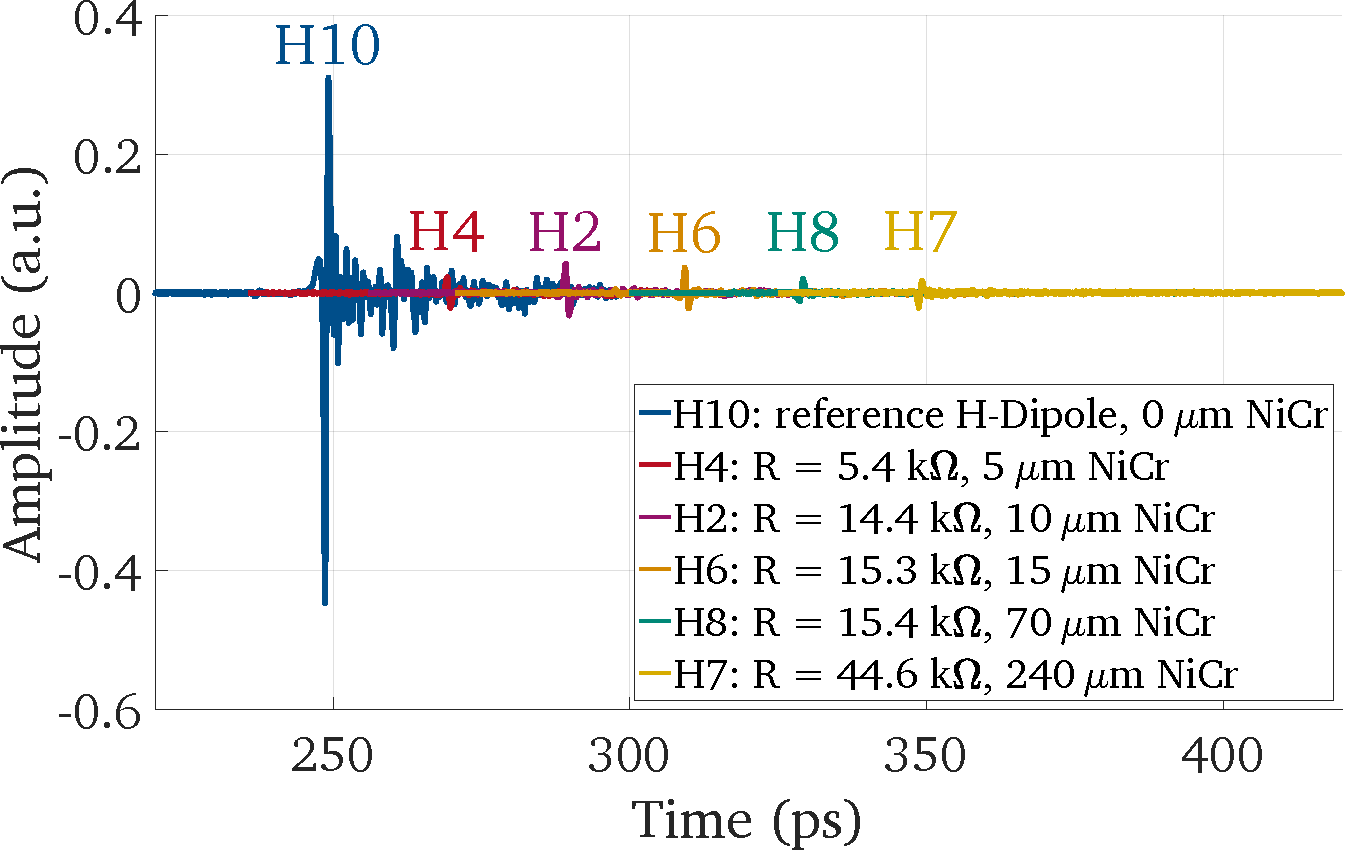
\includegraphics[height=0.6\textwidth]{figures/Results/mainTextComp/comp_H_Dipoles_time.pdf}
        \caption{\centering}
        \label{comp_amp_HD}
    \end{subfigure}
    \hfill
    \begin{subfigure}[b]{0.49\textwidth}
        \centering
        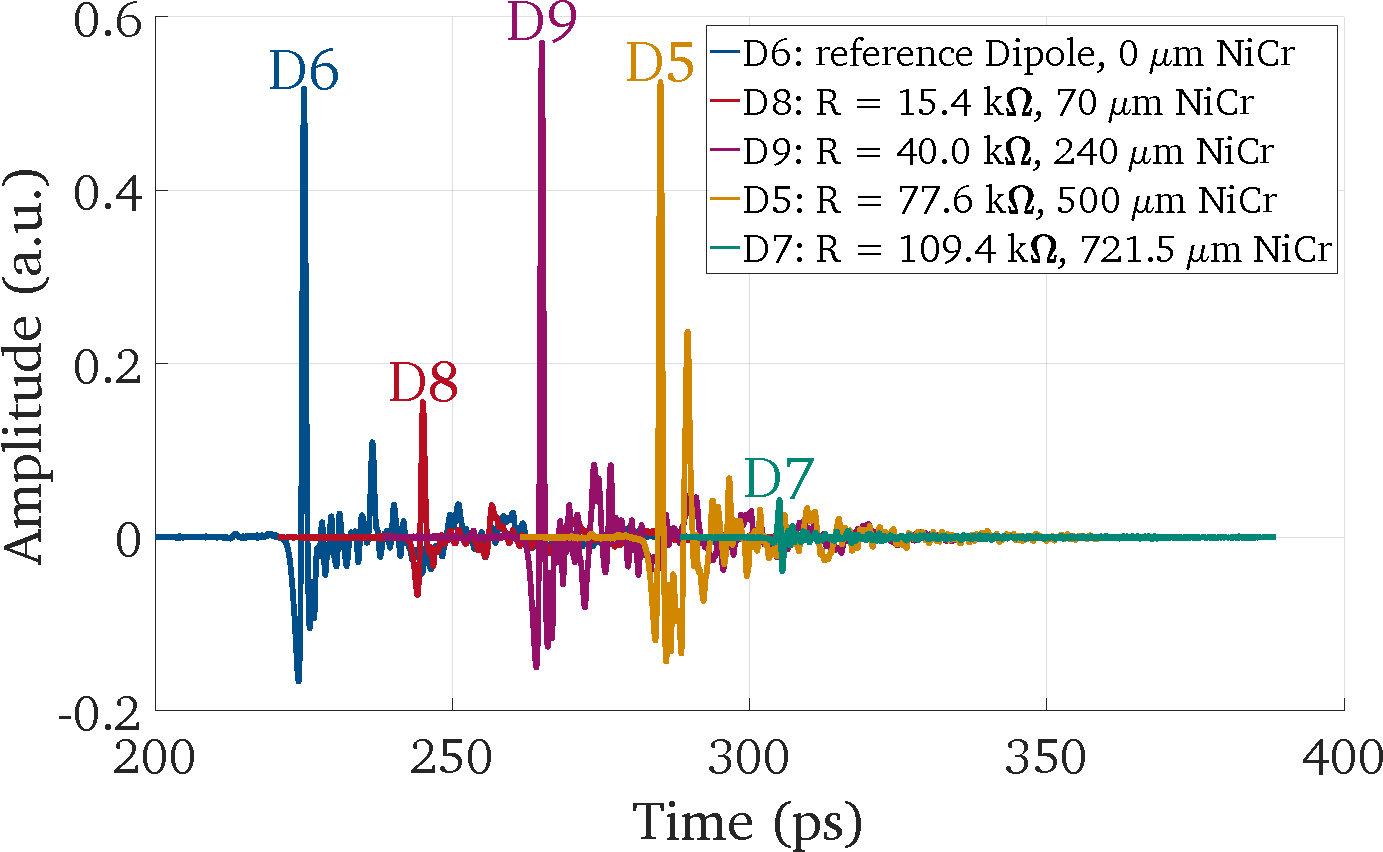
\includegraphics[height=0.6\textwidth]{figures/Results/mainTextComp/comp_Dipoles_time.pdf}
        \caption{\centering}
        \label{comp_amp_D}
    \end{subfigure}
    \caption{Measured time-domain traces of the receives THz pulses. The data is temporally aligned for better comparison of the pulses. (a) Time-domain data of the processed H-Dipole antennas. The NiCr-modified H-Dipoles differ vastly from the reference antenna concerning their measured amplitude. (b) Time-domain data of the processed I-shaped Dipole antennas. Differences in measured amplitude mainly stems from differences in alignment.}
    \label{comp_antenna_amp}
\end{figure}

Figure~\ref{comp_antenna_amp} shows the time-domain measurements for six H-Dipole antennas (see \ref{comp_amp_HD}) and five I-shaped Dipole antennas (see \ref{comp_amp_D}) with different NiCr modifications. The measured data has been temporally aligned so that the measured THz pulses in the plot are spaced apart by \num{20} \si{\pico \s} for better comparison.  

Incorporating NiCr into an H-Dipole antenna reduces the amplitude of the received signal by approx. one order of magnitude. The reference antenna H10, which has no NiCr in the feeding strip, shows an amplitude of \num{0.45}. In contrast, even a very short NiCr segment of \num{5} \si{\micro\meter} in antenna H4 results in significant damping, with a maximum amplitude of only \num{0.025}. This substantial attenuation is most likely caused by the highly resistive NiCr segment, which introduces a dissipative element into the H-Dipole’s feeding strip. Even for the short segment of \num{5} \si{\micro \meter}, the resistance is \num{6.0} \si{\kilo \ohm}. The resulting amplitude reduction worsens the DNR of the antennas. The noise levels in the antennas seem to be similar. For the other NiCr-modified H-Dipole antennas, a longer NiCr segment is generally associated with greater signal loss. The antenna with the longest NiCr strip, measuring \num{240} \si{\micro\meter} (H7), exhibits the highest resistance of \num{44.6} \si{\kilo\ohm} and one of the lowest measured amplitudes at \num{0.021}. Variations in measured amplitude can also be influenced by experimental alignment. The fact that H4 and H7 show nearly identical amplitudes despite their large difference in NiCr length is attributable to such alignment effects.

The effect of signal loss caused by incorporating NiCr into the antenna does not appear to be as severe in I-shaped Dipole antennas. Differences in measured amplitudes of the received signal seem to arise primarily from variations in alignment. D9, with a resistance of approx. \num{131.7}\,\si{\kilo \ohm}, displays a higher amplitude than the reference Dipole D6. Thus, the highly resistive NiCr segment appears to not primarily influence the signal's amplitude. In terms of SNR, the antennas do not show major differences. However, for D5 and D7, which have the highest resistances of \num{274.5}\,\si{\kilo \ohm} and \num{396.0}\,\si{\kilo \ohm}, respectively, the DNR is slightly reduced. The measurements experience noisier signals. 

One reason why the NiCr segments have a more pronounced effect on H-Dipoles than on I-shaped Dipoles is the difference in segment placement. In H-Dipoles, the NiCr segments start at the antenna’s electrodes, whereas in I-shaped Dipoles they start at the antenna’s pads. The placement of the NiCr segments influences the radiation behavior of the antennas. This influence needs to be investigated further through simulations and experimental measurements.

\subsection{Effect of NiCr on THz Performance in H-Dipoles and I-Shaped Dipoles}

The effect of NiCr on the THz performance of the fabricated antennas is investigated by comparing NiCr-modified H-Dipole and I-Shaped Dipole antennas to their respective reference devices. Antenna comparisons are performed by analyzing the measured signals in the time domain as well as the spectra calculated from these measurements. In the time domain, our primary focus is the observation of time-harmonic oscillations. By analyzing the spectra, we gain insight into an antennas’ DNR, roll-off, and bandwidth. 

We analyze the time-domain oscillations caused by non-radiating reflections within the feeding strip. The time-domain data is temporally aligned to facilitate comparison of these oscillations. Additionally, a digital low-pass filter, namely a moving average (MA) filter, is applied to the time-domain traces. The signals are normalized to their respective amplitudes. Averaging and normalizing the data is particularly helpful for noisy signals, as it allows the oscillations caused by strip reflections to be extracted from the noise. These post-processing steps may distort the absolute amplitude information, potentially exaggerating oscillation amplitudes compared to raw measurements. However, this is acceptable for this work, since our primary focus is on the relative influence of NiCr on the oscillations compared to the reference antennas.

The spectra are obtained by calculating the FFT of a measured time-domain trace. To compare performance factors such as bandwidth and DNR, the individual spectra are normalized to their respective noise levels. The noise level of a signal is determined by averaging the spectrum over the range from \num{4}\,\si{\tera \hertz} to \num{6}\,\si{\tera \hertz}. A MA filter is applied to the normalized signal to facilitate evaluation of the bandwidth. Averaging the spectrum improves differentiation between actual signal and noise. The magnitude of the spectra is displayed on a logarithmic scale. Since the received THz power is proportional to the square of the measured photocurrent, the spectra are calculated as follows: $P_{dB} = 20\log_{10}(I_{Ph})$. By normalizing the spectrum to its noise floor, we effectively calculate the DNR of the signal yielding $P_{DNR} = 20\log_{10}(I_{Ph}/I_{noise})$.   

\subsubsection{H-Dipole Measurement Results}

Figure \ref{comp_h10_h4_h2_h6_time} presents the time-domain measurements of the reference H-Dipole (H10) alongside antennas with only small segments of NiCr (H2: \num{10}\,\si{\micro \meter}, H4: \num{5}\,\si{\micro \meter}, and H6: \num{15}\,\si{\micro \meter}). The spectra of antennas H10, H2, H4 and H6 are displayed in Figure \ref{comp_h10_h4_h2_h6_spectum}. Figure \ref{comp_h10_h8_h7_time} shows the time-domain data of the reference H-Dipole antenna (H10) and antennas with larger NiCr segments (H7: \num{70}\,\si{\micro \meter}, H8: \num{240}\,\si{\micro \meter}). The spectra of antennas H10, H7 and H8 are displayed in Figure \ref{comp_h10_h8_h7_spectrum}. 

The reference antenna (H10) shows the best THz performance. Since the entire antenna structure is fabricated from CrAu, no signal is lost due to dissipative elements, as occurs in the other antennas where NiCr is added. H10 does not display the heavy resonant behavior at low frequencies that would normally be expected. Only when averaging the data to improve SNR, some time-harmonic oscillations can be observed. The absence of these major  resonances is primarily due to the THz source in the THz-TDS setup, which is itself an H-Dipole antenna but with a different strip length. The source has a strip length of $l_{strip} = 2300$ \si{\micro\meter}. The H-Dipoles fabricated in this work are designed with $l_{strip} = 1900$ \si{\micro\meter}. Both emitter and detector exhibit resonances at low THz frequencies, caused by standing waves in the antenna strip (see Section \ref{sec:padResonances}). The effective wavelength of these standing waves is proportional to the strip length. Thus, the resonance frequencies differ slightly between the source and H10 and are partially offset \cite{nandiErAsInAlGaAsPhotoconductors2021}. As a result, H10 demonstrates a largely non-resonant response as can be observed in the frequency-domain. Partially due to its high SNR and DNR of \num{52}\,\si{\decibel}, H10 shows a high bandwidth of \num{4.1}\,\si{\tera \hertz}. 

The antennas with short NiCr segments (H2, H4, H6) exhibit very similar THz performances. This is expected, as they only differ slightly in NiCr lengths (\num{10}\,\si{\micro\meter}, \num{5}\,\si{\micro\meter}, and \num{15}\,\si{\micro\meter}, respectively) and resistances (\num{5.4}\,\si{\kilo\ohm}, \num{14.4}\,\si{\kilo\ohm}, and \num{15.3}\,\si{\kilo\ohm}, respectively). The normalized and averaged time-domain traces (see Figure \ref{comp_h10_h4_h2_h6_time}) reveal noticeably noisy signals, which can be attributed to the strong damping of the THz pulses by the NiCr segments. Unlike in H10, the standing-wave oscillations are very present in the time domain. Oscillating waves with a duration of approx. \num{15}\,\si{\pico \s} to \num{20}\,\si{\pico \s} are observable, especially in H4. The oscillations in H2 and H6 are very similar concerning their phase and amplitude. Phase shifts between the reference antenna (H10) and the NiCr-modified antennas (H2, H4, H6) are observed. These phase shifts occur wherever the time-harmonics of the reference antenna exhibit a maximum, while the corresponding time-harmonics in H2, H4, and H6 show a minimum. The cause of these phase shifts, particularly the influence of NiCr on these phase shifts, requires further investigation.
\begin{figure}[!]
    \centering
    \begin{subfigure}[b]{0.49\textwidth}
        \centering
        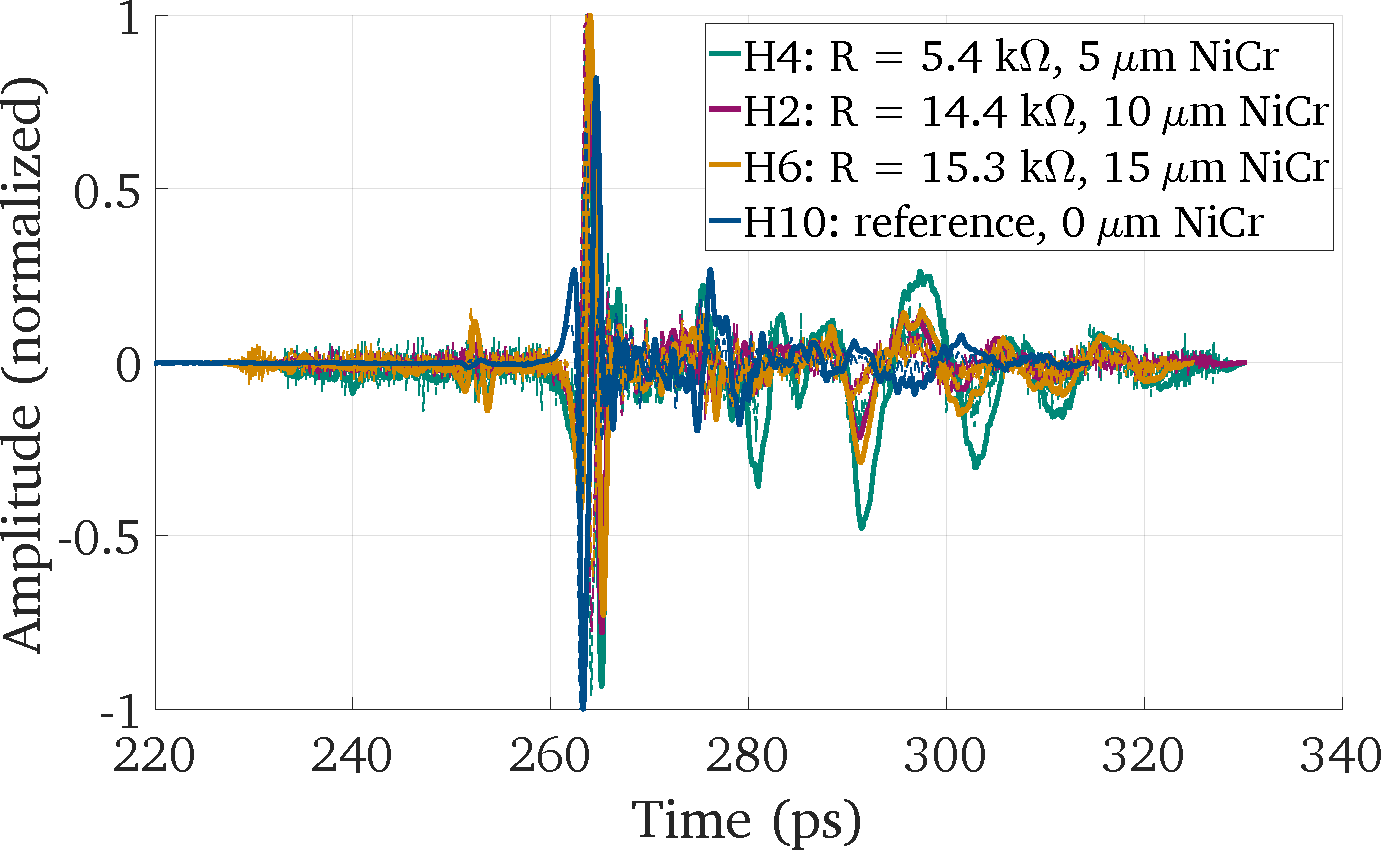
\includegraphics[height=0.6\textwidth]{figures/Results/mainTextComp/H10_H4_H2_H6/H10_H4_H2_H6_MA_time_normed.pdf}
        \caption{\centering}
        \label{comp_h10_h4_h2_h6_time}
    \end{subfigure}
    \hfill
    \begin{subfigure}[b]{0.49\textwidth}
        \centering
        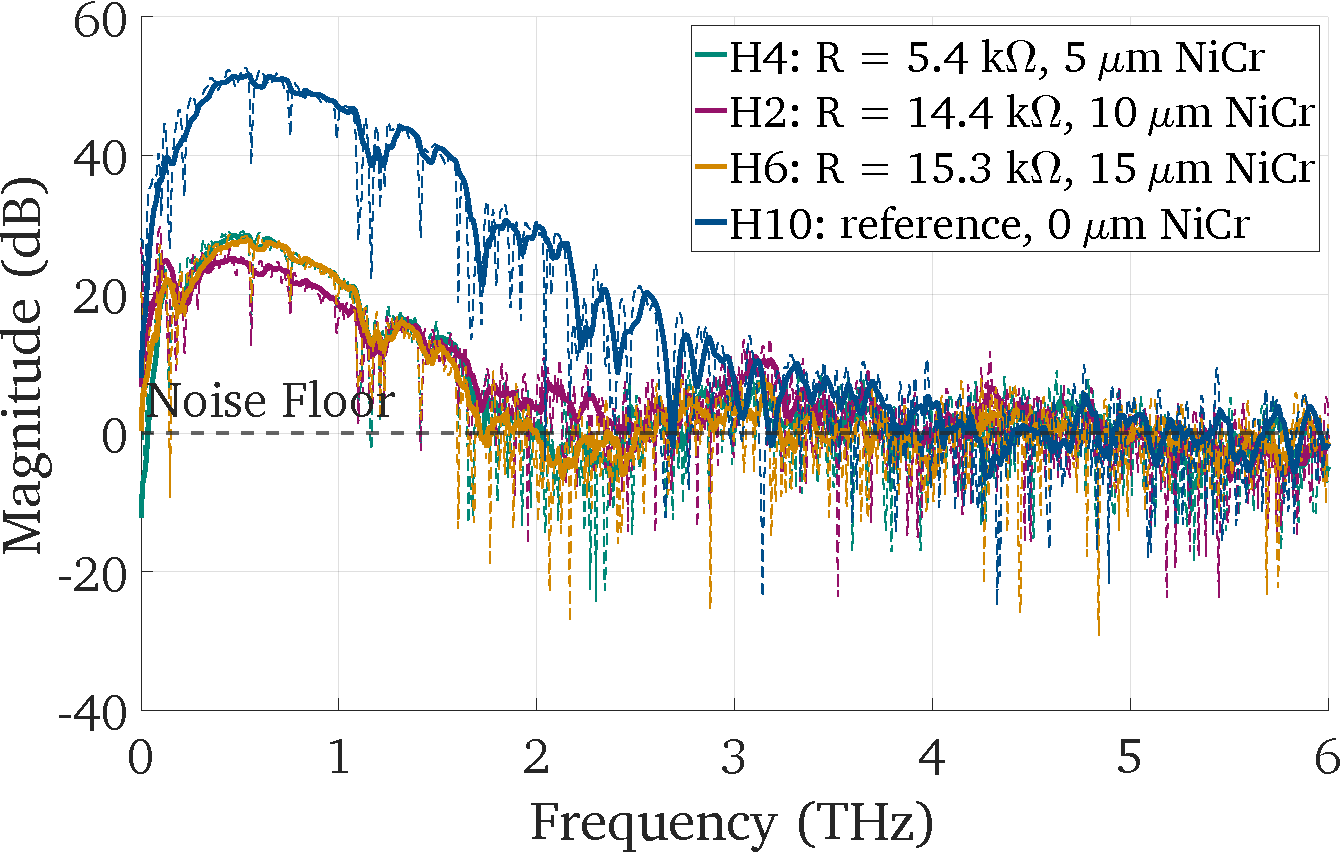
\includegraphics[height=0.6\textwidth]{figures/Results/mainTextComp/H10_H4_H2_H6/H10_H4_H2_H6_spectrum_nn.pdf}
        \caption{\centering}
        \label{comp_h10_h4_h2_h6_spectum}
    \end{subfigure}
    \hfill
    \centering
    \begin{subfigure}[b]{0.49\textwidth}
        \centering
        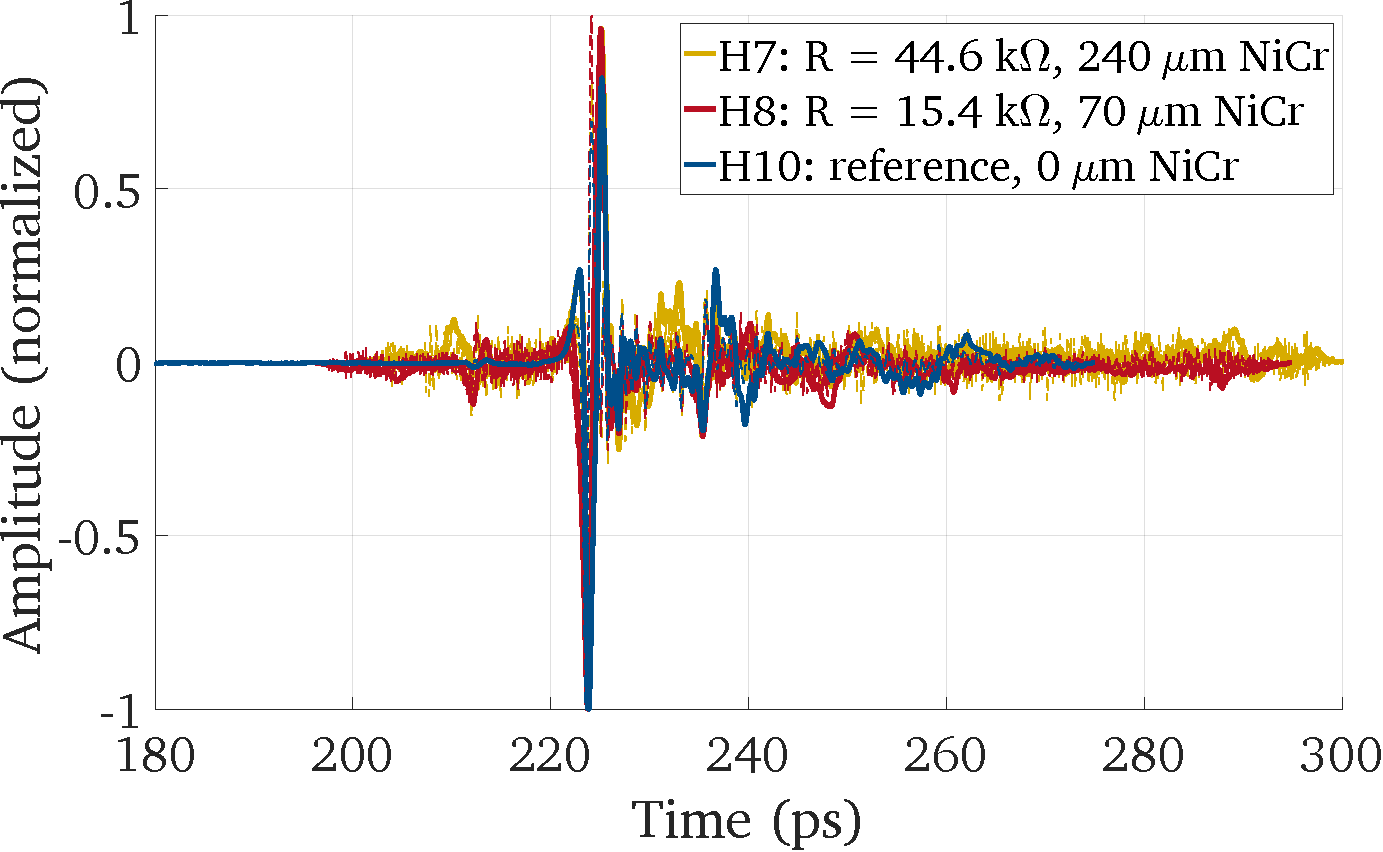
\includegraphics[height=0.6\textwidth]{figures/Results/mainTextComp/H10_H8_H7/H10_H8_H7_MA_time_norm.pdf}
        \caption{\centering}
        \label{comp_h10_h8_h7_time}
    \end{subfigure}
    \hfill
    \begin{subfigure}[b]{0.49\textwidth}
        \centering
        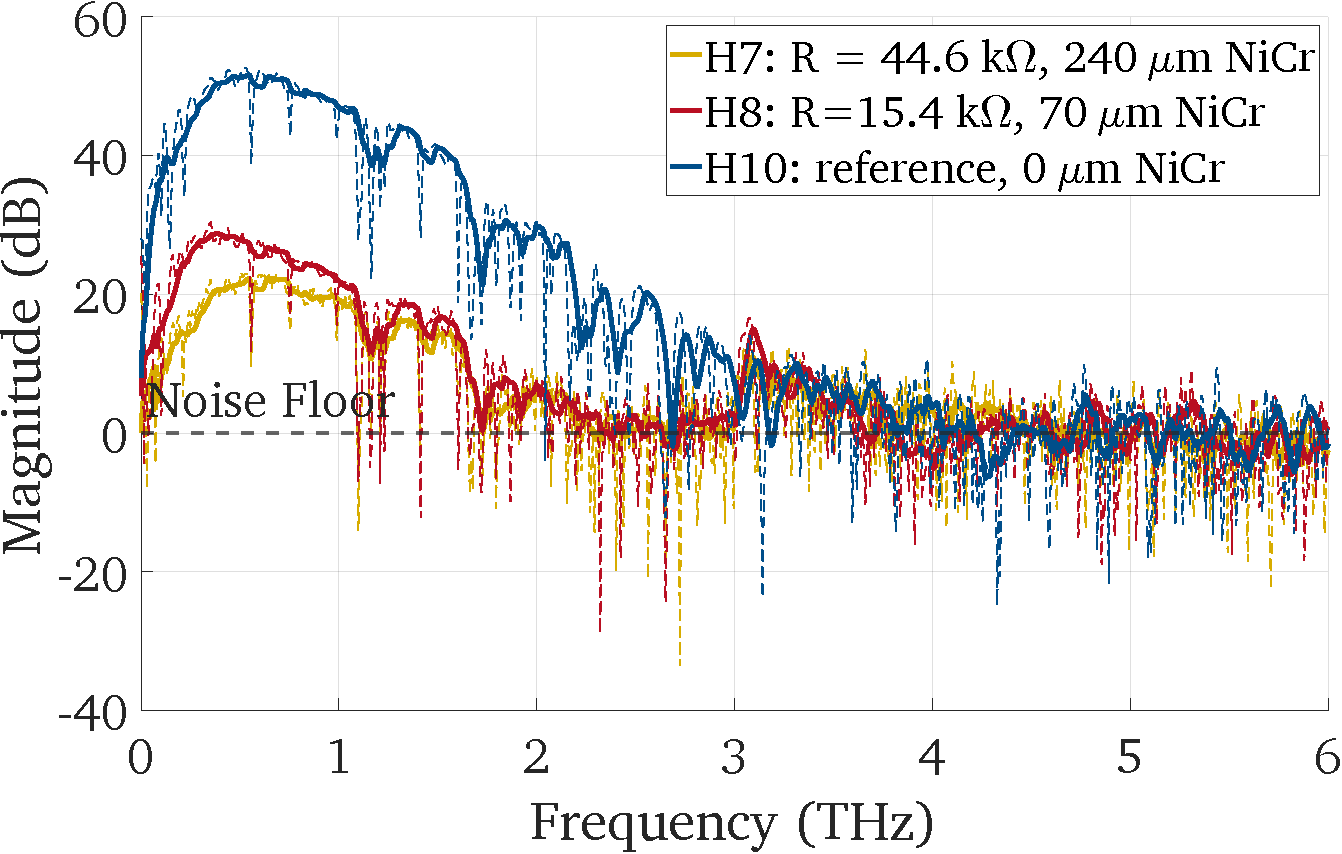
\includegraphics[height=0.6\textwidth]{figures/Results/mainTextComp/H10_H8_H7/H10_H8_H7_spectrum_nn.pdf}
        \caption{\centering}
        \label{comp_h10_h8_h7_spectrum}
    \end{subfigure}
    \caption{THz-TDS measurements showing the received signal in the processed H-Dipole antennas and their corresponding spectra obtained by taking the FFT of the measured signals. A moving average (MA) filter is applied to the data. The original, normalized data are displayed as dotted lines. The time-domain data are normalized to each signal’s amplitude, and the spectra are normalized to their respective noise floors. (a) Normalized, filtered time-domain data for antennas H2, H4, and H6 compared to the reference antenna H10. (b) Normalized, filtered spectra obtained from the measured time-domain traces of antennas H2, H4, H6, and H10. (c) Normalized, filtered time-domain data for antennas H7 and H8 compared to the reference antenna H10. (d) Normalized, filtered spectra obtained from time-domain traces of antennas H7, H8, and H10.}
    \label{comp_dipoles}
\end{figure}

In the frequency domain (see Figure \ref{comp_h10_h4_h2_h6_spectum}), antennas H2, H4 and H6 exhibit a resonance near \num{87}\,\si{\giga\hertz}, matching well with the simulated radiation impedance of an H-Dipole antenna without NiCr. This is notable, as the NiCr segment resistances should, in principle, be sufficient to suppress such resonances. The presence of this resonance suggests that, in addition to a segment’s resistance, its length also plays a role in suppressing low-frequency resonances. As previously discussed, the standing waves in the THz source and in the reference H-dipole (H10) partially cancel due to their different strip lengths (\num{2300}\,\si{\micro\meter} and \num{1900}\,\si{\micro\meter}, respectively). H2, H4, and H6 share the same total strip length as H10 of \num{1900}\,\si{\micro\meter}. Introducing a different material into the strip may alter the reflection of non-radiating waves, enabling these resonances. Another possible explanation is that the NiCr segments shift the resonance frequencies of the receiving antennas. Simulations (see Section \ref{sec:sim_results}) indicate that apart from a resonance approaching extremely low THz frequencies, NiCr-modified antennas are expected to be largely non-resonant. The THz source however still exhibits low-frequency peaks, which could be mirrored into the receiver. Thus, the observed \num{87}\,\si{\giga\hertz} peak may simply originate from a source resonance coupled to the measurement. 

Antennas H4 and H6 exhibit nearly identical bandwidths of approx. \num{2.0}\,\si{\tera \hertz} and a DNR of \num{28}\,\si{\decibel} each, while antenna H2 shows a slightly lower DNR of \num{25}\,\si{\decibel} but higher bandwidth of \num{2.28}\,\si{\tera\hertz}. The differences in bandwidth and DNR for H2, H4 and H6 are likely due to slight variations in alignment. Note that the peak happening in the spectrum around \num{3.1}\,\si{\tera \hertz} may be discarded as an artifact caused by noise in the measurement setup.

The H-Dipoles with larger NiCr segments (H7, H8) differ concerning their THz performances. Both antennas have a bandwidth of approx. \num{2.6}\,\si{\tera \hertz}. However, H7 exhibits a DNR of \num{24}\,\si{\decibel}, H8 has a DNR of \num{30}\,\si{\decibel}. A difference of \num{6}\,\si{\decibel} corresponds to approx. twice the amount of signal received in H8. This behavior is expected as power and resistance should be proportional and the resistance of H7 is approx. three times the resistance of H8. Compared to H10, both H7 and H8 seem to show a flatter trend, meaning their roll-off is less severe. RC roll-off and lifetime roll-off should be identical for all processed antennas. All antennas sit on the same semiconducting material and their electrodes are configured identically. The addition of NiCr to the H-Dipole seems to impact the overall antenna roll-off positively. A flat behavior of the antennas, especially observable in H7 may be beneficial in some applications. 

The low-frequency resonances observable in H2, H4, and H6 are absent in the spectra of antennas H7 and H8, which have NiCr strips of length \num{240}\,\si{\micro \meter} and \num{70}\,\si{\micro \meter}, respectively. In the normalized and averaged time-domain traces (see Figure \ref{comp_h10_h8_h7_time}), we observe that the time-harmonic oscillations are significantly damped compared to those in H10, where they were already quite suppressed. H8 exhibits some low frequency oscillations between \num{240}\,\si{\pico \s} and \num{270}\,\si{\pico \s}. The duration of this oscillation corresponds to a frequency of approx. \num{60}\,\si{\giga \hertz}. At \num{60}\,\si{\giga \hertz}, a small resonant peak is observable in the spectrum (see Figure \ref{comp_h10_h8_h7_spectrum}). A vast amount of oscillations seems to be damped by the NiCr segments, which is especially observable for H7, which has the largest resistance and NiCr strip length. After \num{250}\,\si{\pico \s}, the normalized and averaged data is indistinguishable from noise. In the reference (H10), we can still observe low frequency harmonics at this time. The observations made in the time-domain can be confirmed by examining the corresponding spectrum (see Figure \ref{comp_h10_h8_h7_spectrum}). Unlike antennas H2, H4, and H6, antennas H7 and H8 do not exhibit a significant resonant peak before reaching their maximum magnitude. Again, the peak in the spectrum happening around \num{3.1}\,\si{\tera \hertz} may be discarded as an artifact.

Comparing all H-Dipoles, we notice that H7 and H8 with resistances of \num{44.6}\,\si{\kilo \ohm} and \num{15.4}\,\si{\kilo \ohm} respectively exhibit higher bandwidths than antennas H2, H4 and H6 with resistances of \num{14.4}\,\si{\kilo \ohm}, \num{5.4}\,\si{\kilo \ohm} and \num{15.3}\,\si{\kilo \ohm} respectively. This indicates that NiCr does not significantly impact an antenna’s performance at higher frequencies. Variations in antenna alignment may cause differences in bandwidth, explaining why some antennas experience noise earlier. The bandwidth of the NiCr-modified antennas seems primarily affected by their lower SNR compared to the reference antenna. While this reduced SNR results from the introduction of NiCr, it could be mitigated by packaging the antennas and improving measurement alignment. We demonstrated that with good alignment, NiCr-modified H-dipoles exhibit a less severe roll-off compared to the reference antenna. With proper packaging, similar bandwidths to the reference could be achieved, while maintaining a relatively flat and non-resonant response at lower THz frequencies.

\subsubsection{I-Shaped Dipole Measurement Results}

% \begin{itemize}
%     \item less severe roll-off in NiCr modified I-shaped Dipoles 
%     \item once again: low-f resonances because of emitter resonances 
%     \item maybe say something about expected resonances of the Dipoles 
%     \item D5 has largest BW for some reason; probably alignment 
%     \item D9 also has larger BW than reference; in combination with D5: NiCr definitely does not impact BW negatively, high frequencies not effected at all (at least until a certain maximum amount of NiR) + flatter roll-off !!!!
%     \item once again: alignment, packaging 
% \end{itemize}

Figure \ref{comp_d6_d8_d9_time} presents the time-domain data of the reference I-shaped Dipole (D6) alongside antennas D8 and D9, featuring NiCr sections of length \num{70}\,\si{\micro \meter} and \num{240}\,\si{\micro \meter} respectively. The spectra of antennas D6, D8 and D9 are displayed in Figure \ref{comp_d6_d8_d9_time}. Figure \ref{comp_d6_d5_d7_time} shows the time-domain traces of the reference I-shaped Dipole (D6) alongside antennas D5 and D7, featuring NiCr segments of length \num{500}\,\si{\micro \meter} and \num{721.5}\,\si{\micro \meter} respectively. The spectra of antennas D6, D5 and D7 are displayed in Figure \ref{comp_d6_d5_d7_spec}.

The I-shaped Dipole used as a reference (D6) displays time-harmonic oscillations visible after reception of the main THz pulse (see Figure \ref{comp_d6_d8_d9_time}). The resonant peaks appear to be spaced apart by approx. \num{14}\,\si{\pico \s}, corresponding to a frequency of approx. \num{35}\,\si{\giga \hertz}. Oscillations at multiples of this frequency fit well with simulations and the obtained spectrum from measurements. Simulations of the radiation impedance of I-shaped Dipoles (see appendix) predicted resonances to occur at \num{37}\,\si{\giga \hertz}, \num{108}\,\si{\giga \hertz} and \num{182}\,\si{\giga \hertz}, all of which can be confirmed by looking at the obtained spectrum of D6 (see \ref{comp_d6_d8_d9_spec}). Additionally, a resonant spike at \num{87}\,\si{\giga \hertz} may be attributed to mirroring of a resonance from the THz source to the receiver, as explained earlier. D6 exhibits a bandwidth of \num{2.6}\,\si{\tera \hertz} and a DNR of \num{64}\,\si{\decibel}. 

Time-harmonic oscillations are present in the time-domain traces of antennas D8 and D9 (\num{70}\,\si{\micro \meter} NiCr and \num{240}\,\si{\micro \meter} NiCr, respectively). The NiCr segments exhibit resistances of \num{38.4}\,\si{\kilo \ohm} for D8 and \num{131.7}\,\si{\kilo \ohm} for D9. These resistive NiCr segments do not sufficiently damp the resonant oscillations following the main THz pulse. The reference I-shaped Dipole (D6) shows its dominant resonance accompanied by higher-frequency harmonics at integer multiples of that frequency. The spectra of D8 and D9 are dominated almost entirely by their primary low-frequency resonance, with higher-order harmonics being largely suppressed by the incorporation of NiCr. In D8, a phase shift occurs at approx. \num{260}\,\si{\pico \s}. The phase of D9 follows that of the reference I-shaped Dipole. The influence of the incorporation NiCr segments on phase behavior requires further investigation.

The observed oscillations in the normalized, averaged time-domain data of antennas D8 and D9 correspond to resonant peaks in the spectra (see Figure \ref{comp_d6_d8_d9_spec}) of the respective devices. Antenna D9 exhibits resonances at \num{100}\,\si{\giga \hertz} and \num{200}\,\si{\giga \hertz}, as well as a resonance at \num{87}\,\si{\giga \hertz}, which is attributed to a mirroring effect from the THz source. Antenna D8 exhibits a dominant resonance at \num{80}\,\si{\giga \hertz}, followed by smaller resonant peaks spaced approx. \num{80}\,\si{\giga \hertz} apart. No source mirroring is observed in antenna D8. The observed resonances match well with simulations.

Concerning THz performance, D8 and D9 behave similarly. The peak DNR is \num{55}\,\si{\decibel} for D8 and \num{53}\,\si{\decibel} for D9. Both antennas exhibit a bandwidth of approx. \num{2.7}\,\si{\tera \hertz}, slightly exceeding the bandwidth of the reference (D6). The peak DNR of D8 and D9 is \num{10}\,\si{\decibel} lower than that of D6, meaning D6 receives three times more THz power at its peak. Despite this, D8 and D9 show a less severe roll-off, resulting in a flatter spectrum and thus slightly higher bandwidth. This effect is especially observed in D9 (\num{240}\,\si{\micro \meter} NiCr). From its peak DNR to \num{1}\,\si{\tera \hertz}, the received signal drops by only \num{13}\,\si{\decibel}. The power received by D6 drops by \num{16}\,\si{\decibel}. At \num{2.2}\,\si{\tera \hertz}, the spectra of D6, D8 and D9 intersect, confirming that the NiCr-modified antennas suppress low-frequency power but leave high-frequency performance largely unaffected.

The THz performance (see Figure \ref{comp_d6_d5_d7_spec}) of I-shaped Dipoles D5 and D7 (NiCr lengths of \num{500}\,\si{\micro \meter} and \num{721.5}\,\si{\micro \meter}, respectively) differs significantly. D5 shows a peak DNR of \num{67}\,\si{\decibel}, exceeding that of the reference (D6). The peak DNR of D7 is \num{35}\,\si{\decibel}. The maximum THz power received by antenna D7 is only \num{1}/\num{40} of that received by D5 or D6. Less received power in D7 can be attributed to the Dipole arm entirely fabricated from NiCr. Much of the received signal is dissipated. Antenna D7 exhibits a bandwidth of \num{2.7}\,\si{\tera \hertz}, slightly higher than that of the reference (D6) at \num{2.6}\,\si{\tera \hertz}. As with the shorter NiCr segments, the performance loss is concentrated at lower THz frequencies, with higher-frequency reception unaffected. An exceptionally flat spectrum is observed in D7. Between \num{0.2}\,\si{\tera \hertz} and \num{1.5}\,\si{\tera \hertz}, the received Thz power varies by just \num{10}\,\si{\decibel}, compared to \num{25}\,\si{\decibel} in D6. The high DNR of D5 is largely attributed to alignment during measurements. The combination of optimal alignment and reduced roll-off observed in NiCr-modified antennas yield an extended bandwidth of \num{3.8}\,\si{\tera \hertz} compared to \num{2.6}\,\si{\tera \hertz} for the reference. 

The low frequency harmonics (see Figure \ref{comp_d6_d5_d7_time}) that were observed in D6, D8 and D9 (\num{0}\,\si{\micro \meter} NiCr, \num{70}\,\si{\micro \meter} NiCr and \num{240}\,\si{\micro \meter} NiCr, respectively) vanish in antenna D7, where the entire Dipole arm is fabricated from NiCr. In D7, only weak higher-frequency harmonics remain after the main pulse, with no dominant low-frequency oscillation present. The I-shaped Dipole D5 (\num{500}\,\si{\micro \meter} NiCr) exhibits more pronounced time-harmonic oscillations compared to D6, though at higher frequencies. Both D5 and D7 show substantial damping of low-frequency oscillations.

The spectral data confirm the time-domain observations. D5 exhibits resonant peaks at integer multiples of \num{80}\,\si{\giga \hertz}. The peak-to-peak amplitude of these oscillations in the frequency domain is considerably larger than those of the other resonances observed so far. This pronounced modulation is consistent with the large secondary pulse following the primary pulse observed in the time-domain traces of D5. Antenna D7 shows only a single peak at \num{87}\,\si{\giga \hertz}, where the resonance in the THz source is mirrored to the device. corresponding to the mirrored resonance of the THz source. As seen in the time-domain, D7 displays a largely non-resonant response.

All NiCr-modified I-shaped Dipole antennas exhibit an increased bandwidth compared to the reference. The maximum bandwidth of \num{3.8}\,\si{\tera \hertz} was achieved in D5, featuring NiCr segments of length \num{500}\,\si{\micro \meter} and a resistance of approx. \num{274.6}\,\si{\kilo \ohm}. With packaging, the bandwidth of the devices could be further increased. NiCr does not impact the I-shaped Dipoles performance at higher THz frequencies. While the peak DNR decreases in the NiCr-modified devices, roll-off reduces as well. A notably flat antenna response was observed in antenna D7, featuring NiCr segments of length \num{721.5}\,\si{\micro \meter} and a resistance of approx. \num{396.0}\,\si{\kilo \ohm}. Such flat responses over a broad frequency range may prove beneficial in some applications. 

\begin{figure}[!]
    \centering
    \begin{subfigure}[b]{0.49\textwidth}
        \centering
        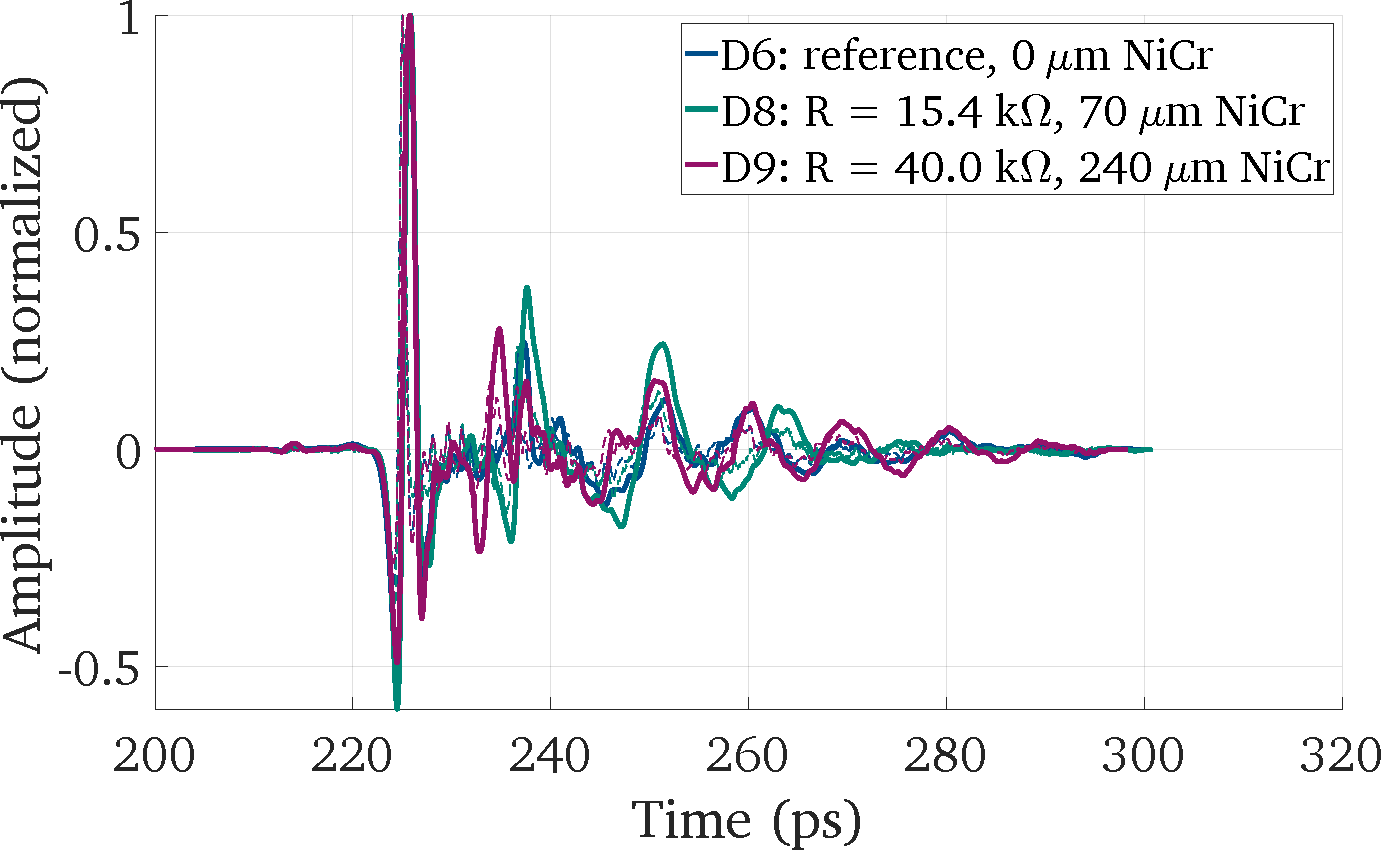
\includegraphics[height=0.6\textwidth]{figures/Results/mainTextComp/D6_D8_D9/D6_D8_D9_MA_time_norm.pdf}
        \caption{\centering}
        \label{comp_d6_d8_d9_time}
    \end{subfigure}
    \hfill
    \begin{subfigure}[b]{0.49\textwidth}
        \centering
        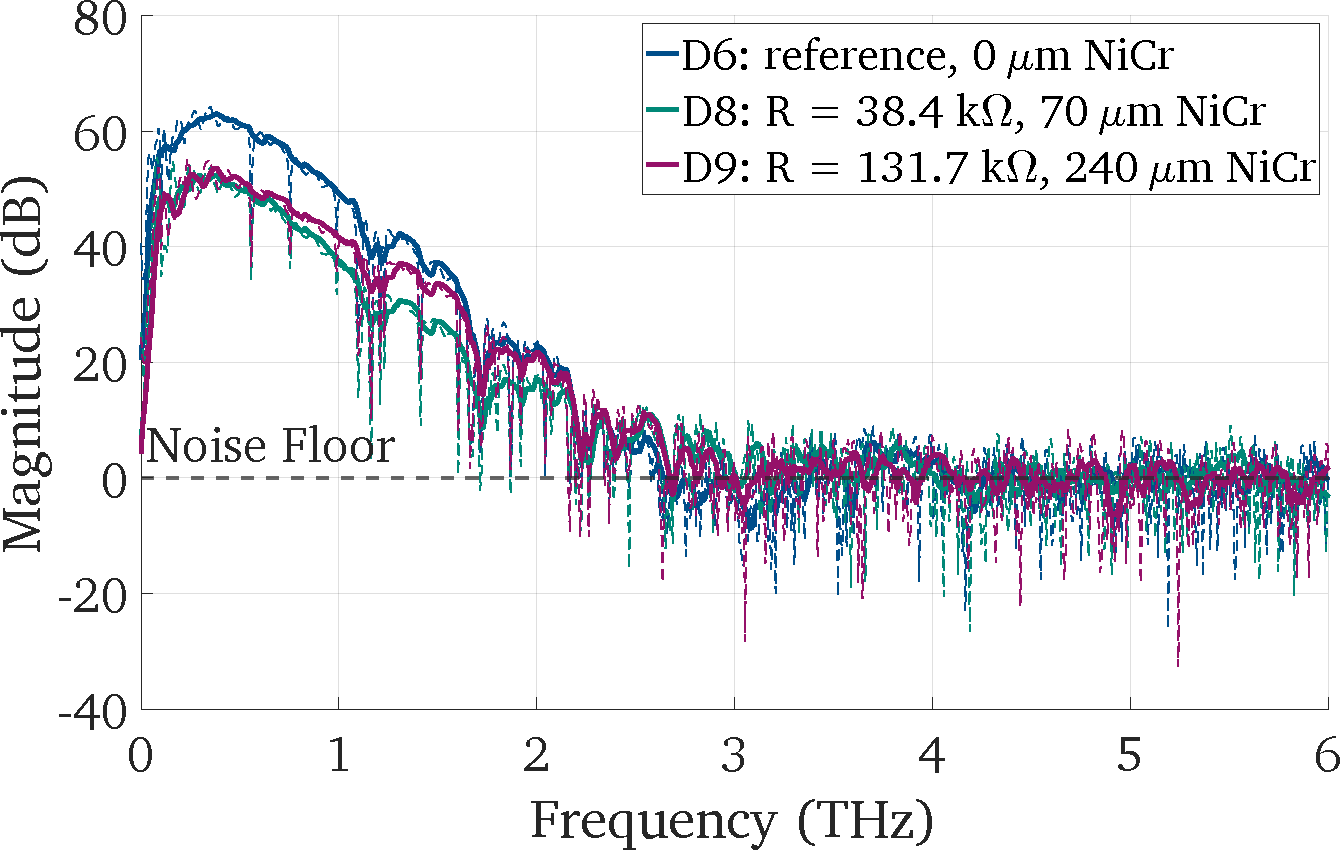
\includegraphics[height=0.6\textwidth]{figures/Results/mainTextComp/D6_D8_D9/D6_D8_D9_spectrum.pdf}
        \caption{\centering}
        \label{comp_d6_d8_d9_spec}
    \end{subfigure}
    \hfill
    \begin{subfigure}[b]{0.49\textwidth}
        \centering
        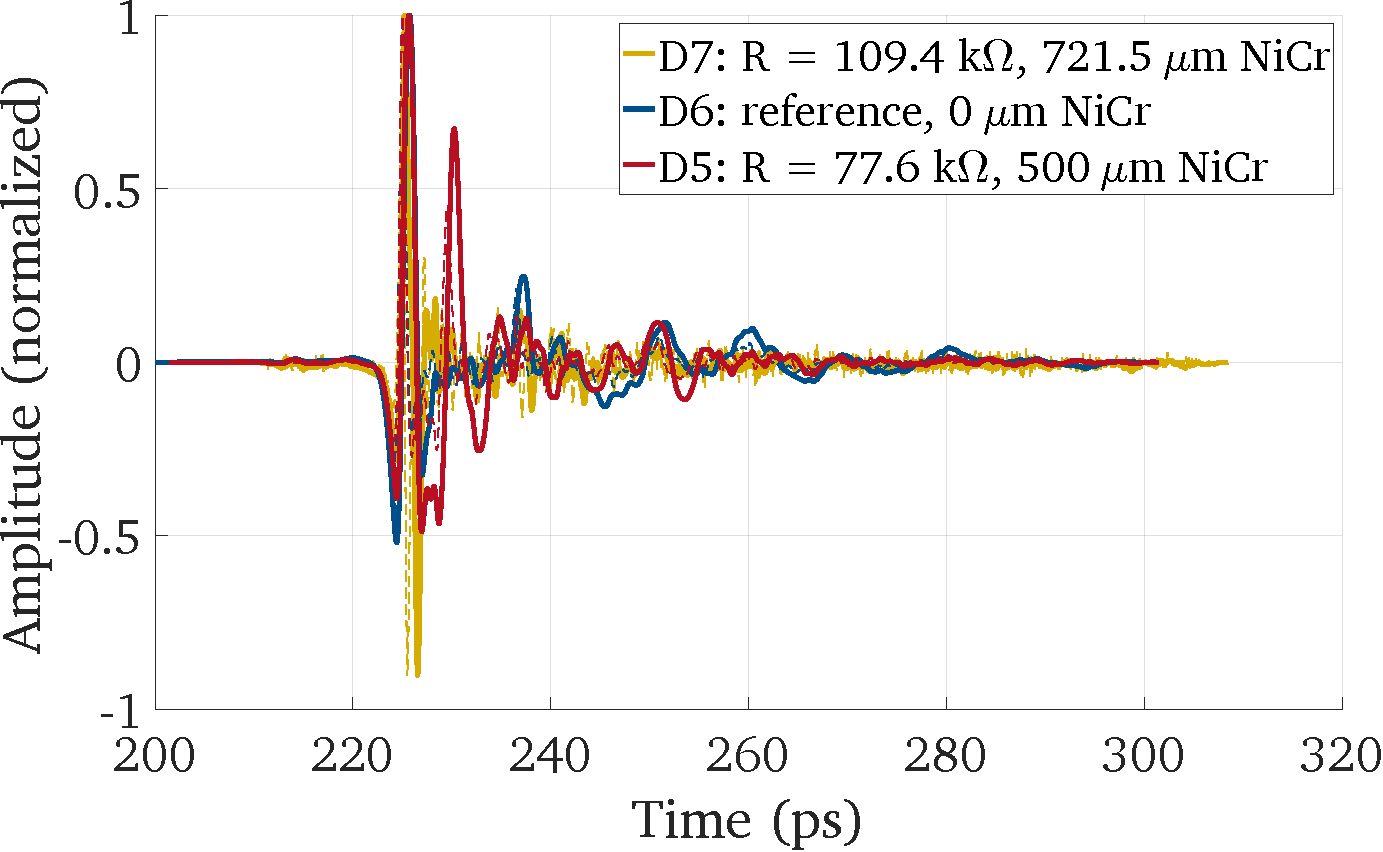
\includegraphics[height=0.6\textwidth]{figures/Results/mainTextComp/D6_D5_D7/D6_D5_D7_MA_time_norm.pdf}
        \caption{\centering}
        \label{comp_d6_d5_d7_time}
    \end{subfigure}
    \hfill
    \begin{subfigure}[b]{0.49\textwidth}
        \centering
        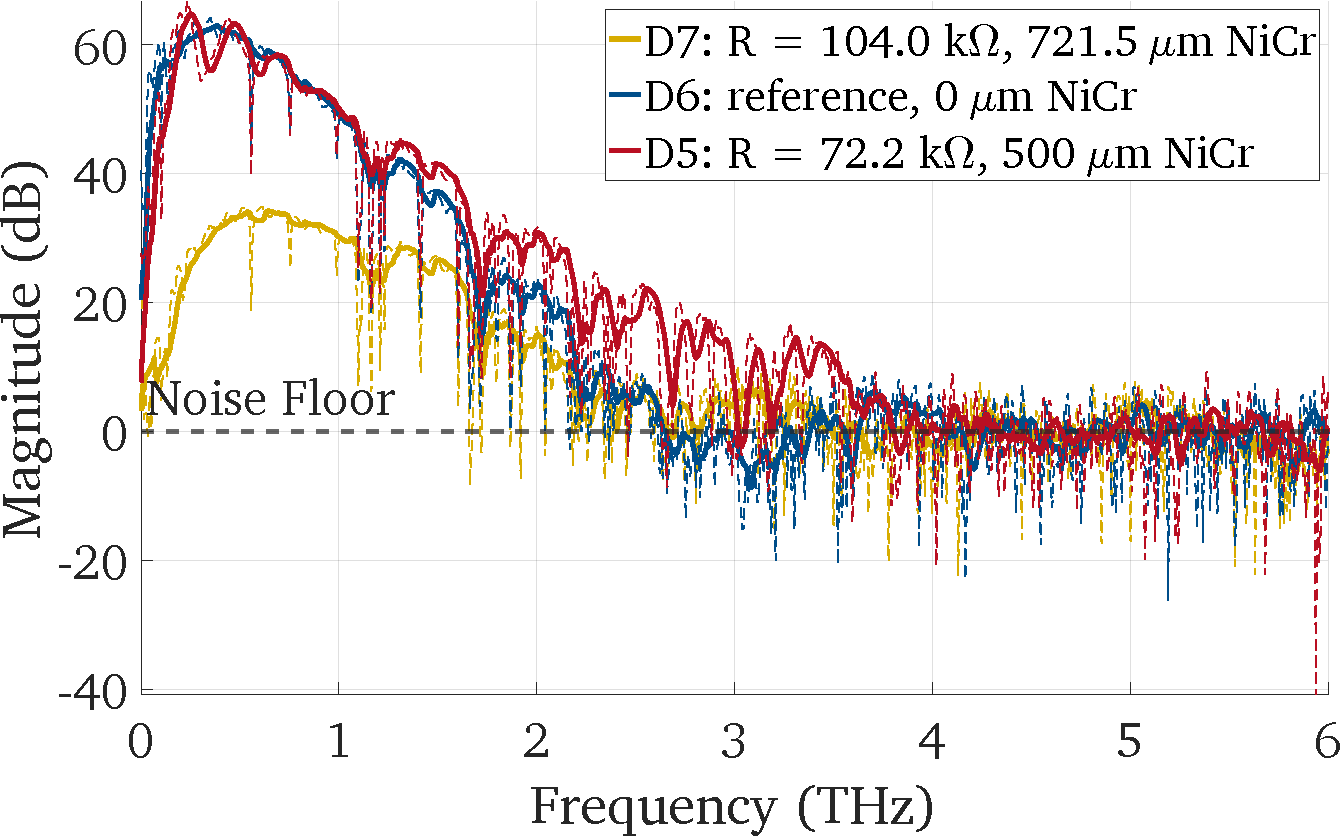
\includegraphics[height=0.6\textwidth]{figures/Results/mainTextComp/D6_D5_D7/D6_D5_D7_spectrum.pdf}
        \caption{\centering}
        \label{comp_d6_d5_d7_spec}
    \end{subfigure}
    \caption{THz-TDS measurements showing the received signal in the processed I-shaped Dipole antennas and their corresponding spectra obtained by taking the FFT of the measured signals. A moving average (MA) filter is applied to the data. The original, normalized data are displayed as dotted lines. The time-domain data are normalized to each signal’s amplitude, and the spectra are normalized to their respective noise floors. (a) Normalized, filtered time-domain data for antennas D8 and D9 compared to the reference antenna D6. (b) Normalized, filtered spectra obtained from the measured time-domain traces of antennas D8, D9 and D6. (c) Normalized, filtered time-domain data for antennas D5 and D7 compared to the reference antenna D6. (d) Normalized, filtered spectra obtained from time-domain traces of antennas D5, D7 and D6.}
    \label{comp_I_dipoles}
\end{figure}

% \subsection{Comparison of H-Dipole, I-Shaped Dipole and Long I-Shaped Dipole}

% \begin{figure}[ht]
%     \centering
%     \begin{subfigure}[b]{0.49\textwidth}
%         \centering
%         \includegraphics[height=0.6\textwidth]{figures/Results/mainTextComp/D6_H10_D1.1/D6_H10_D1.1_MA_time_norm.pdf}
%         \caption{\centering}
%     \end{subfigure}
%     \hfill
%     \begin{subfigure}[b]{0.49\textwidth}
%         \centering
%         \includegraphics[height=0.6\textwidth]{figures/Results/mainTextComp/D6_H10_D1.1/D6_H10_D1.1_spectrum.pdf}
%         \caption{\centering}
%     \end{subfigure}
%     \caption{}
% \end{figure}